\subsection{状態変数}

伝達関数は入力から出力への関係をよく表すが、内部の量を直接扱いたいときには状態空間表現が必要になる。状態空間表現では、対象の過去の履歴をすべて覚えておく代わりに、時刻 $t$ の状態ベクトル $x(t)$ に必要な情報を集める。入力 $u(t)$ を与えれば、次の瞬間の状態変化 $\dot{x}(t)$ と出力 $y(t)$ が現在の $x(t)$ と $u(t)$ から決まる、という因果構造を式にする。

有限次元の連続時間線形時不変系を考える。状態 $x(t)\in\R^n$、入力 $u(t)\in\R^m$、出力 $y(t)\in\R^p$ に対して、状態方程式と出力方程式は
\begin{align}
  \dot{x}(t)&=Ax(t)+Bu(t),\\
  y(t)&=Cx(t)+Du(t)
  \label{eq:ss}
\end{align}
と書く。ここで
\begin{equation}
  A\in\R^{n\times n},\quad
  B\in\R^{n\times m},\quad
  C\in\R^{p\times n},\quad
  D\in\R^{p\times m}
\end{equation}
である。行列が時刻に依存しないので、同じ状態と同じ入力からは時刻によらず同じ変化率と同じ出力が得られる。この性質を時不変性という。式が $x$ と $u$ の一次結合で書けるので、重ね合わせが成り立つ。この性質を線形性という。

$A$ は自律行列またはシステム行列であり、入力を加えないときに状態同士がどのように結合して変化するかを表す。成分で書けば
\begin{equation}
  \dot{x}_i=\sum_{j=1}^{n}a_{ij}x_j+\sum_{j=1}^{m}b_{ij}u_j
\end{equation}
であるから、$a_{ij}$ は $j$ 番目の状態が $i$ 番目の状態の変化率へ与える係数である。$B$ は入力行列であり、各入力がどの状態方程式へどの強さで入るかを表す。$C$ は出力行列であり、状態のどの組み合わせを測定量または制御したい量として取り出すかを表す。$D$ は直達行列であり、入力が状態の積分を経ずに同じ時刻の出力へ直接現れる成分である。多くの機械系で位置を出力にすると $D=0$ になるが、静的な増幅器、センサの直接項、または入力そのものを出力に含むモデルでは $D\ne0$ になり得る。

外乱やノイズを明示したいときは、例えば
\begin{equation}
  \dot{x}=Ax+Bu+Ew,\qquad y=Cx+Du+v
\end{equation}
のように、外乱 $w$ と測定ノイズ $v$ を分けて書く。本節では状態遷移と制御設計の基本を見やすくするため、まず \weq{ss} の形を中心に扱う。

ベクトルは複数の量を一つの点として扱う記法であり、内積
\begin{equation}
  x^\T y=\sum_{i=1}^{n}x_i y_i
\end{equation}
は向きのそろい具合を表す。ノルム
\begin{equation}
  \norm{x}=\sqrt{x^\T x}
\end{equation}
は状態の大きさを測る。3次元の力学では外積
\begin{equation}
  a\times b=\begin{bmatrix}
    a_2b_3-a_3b_2\\ a_3b_1-a_1b_3\\ a_1b_2-a_2b_1
  \end{bmatrix}
\end{equation}
がモーメントや角運動量に現れる。

行列は線形写像である。ランク $\rank A$ は、行列がどれだけ独立な方向を作れるかを表す。正方行列 $A$ の固有値と固有ベクトルは
\begin{equation}
  Av=\lambda v
\end{equation}
で定義される。状態方程式では、$A$ の固有値が内部モードの速さと振動を決める。

\subsection{行列指数関数と状態遷移行列}

スカラーの微分方程式 $\dot{x}=ax$ の解が $x(t)=e^{a(t-t_0)}x(t_0)$ であるように、入力なしのベクトル微分方程式
\begin{equation}
  \dot{x}=Ax
\end{equation}
の解は行列指数関数で表される。行列指数関数は
\begin{equation}
  e^{A\Delta t}
  =I+A\Delta t+\frac{1}{2!}A^2\Delta t^2+\frac{1}{3!}A^3\Delta t^3+\cdots
  \label{eq:matrix-exponential-definition}
\end{equation}
という冪級数で定義される。右辺の各項はすべて $n\times n$ 行列であり、$I$ は単位行列である。級数定義を使うと、行列指数関数の基本性質はスカラー指数関数と同じ形で確かめられる。
\begin{align}
  e^{A\cdot 0}&=I,\\
  \frac{\dd}{\dd t}e^{A(t-t_0)}&=Ae^{A(t-t_0)}=e^{A(t-t_0)}A,\\
  e^{A(t_2-t_1)}e^{A(t_1-t_0)}&=e^{A(t_2-t_0)},\\
  \left(e^{A(t-t_0)}\right)^{-1}&=e^{-A(t-t_0)}.
\end{align}
ただし、異なる行列が混ざるときは注意が必要である。一般には $AB\ne BA$ なので、$e^{(A+B)t}=e^{At}e^{Bt}$ は成り立たない。これはスカラー指数関数との重要な違いである。

連続時間線形時不変系では
\begin{equation}
  \Phi(t,t_0)=e^{A(t-t_0)}
  \label{eq:state-transition-matrix}
\end{equation}
を状態遷移行列という。状態遷移行列は、時刻 $t_0$ の状態を時刻 $t$ の状態へ写す行列であり、同次系の解は
\begin{equation}
  x_h(t)=\Phi(t,t_0)x(t_0)
  \label{eq:homogeneous-solution}
\end{equation}
である。この $x_h$ を同次解、自然応答、または零入力応答という。入力がないときの状態の減衰、発散、振動は $A$ の固有値によって決まる。$A$ が対角化できて $A=V\Lambda V^{-1}$ なら
\begin{equation}
  e^{A(t-t_0)}=V e^{\Lambda(t-t_0)}V^{-1},\qquad
  e^{\Lambda(t-t_0)}=\diag(e^{\lambda_1(t-t_0)},\ldots,e^{\lambda_n(t-t_0)}).
\end{equation}
したがって、固有値の実部が負なら対応するモードは減衰し、正なら増大し、虚部は振動角周波数として現れる。

入力がある場合、解は同次解と強制解の和になる。時刻 $t_0$ から始めると
\begin{equation}
  x(t)=\Phi(t,t_0)x(t_0)
  +\int_{t_0}^{t}\Phi(t,\tau)Bu(\tau)\,\dd\tau
  \label{eq:ss-solution}
\end{equation}
である。第一項は初期状態だけが作る零入力応答であり、第二項は入力が作る零状態応答である。積分の中の $\Phi(t,\tau)B$ は、時刻 $\tau$ に入力が状態へ加えた小さな変化 $Bu(\tau)\dd\tau$ が、その後 $t$ まで自然運動で運ばれた結果を表す。この形を畳み込み積分という。線形時不変系では $\Phi(t,\tau)=e^{A(t-\tau)}$ なので、現在の状態は過去入力の履歴を重み $e^{A(t-\tau)}B$ で足し合わせたものになる。

出力も同じ分解で表せる。\weq{ss-solution} を出力方程式へ代入すると
\begin{equation}
  y(t)=C\Phi(t,t_0)x(t_0)
  +\int_{t_0}^{t}C\Phi(t,\tau)Bu(\tau)\,\dd\tau
  +Du(t)
  \label{eq:ss-output-solution}
\end{equation}
である。零初期状態なら、入力から出力への動的な核は
\begin{equation}
  g(t-\tau)=Ce^{A(t-\tau)}B
\end{equation}
であり、$D$ は積分を経ない同時刻の項である。伝達関数でいう直達項は、この $D$ に対応する。

\subsubsection{二状態モデルにおける状態遷移}

二つの状態だけをもつ標準的な例として、正規化した質量ばねダンパ系
\begin{align}
  \dot{x}
  &=
  \begin{bmatrix}0&1\\-2&-3\end{bmatrix}x
  +
  \begin{bmatrix}0\\1\end{bmatrix}u,\\
  y&=\begin{bmatrix}1&0\end{bmatrix}x
\end{align}
を考える。$x_1$ は変位、$x_2$ は速度である。第一行 $\dot{x}_1=x_2$ は速度が変位の時間微分であることを表す。第二行 $\dot{x}_2=-2x_1-3x_2+u$ では、$-2x_1$ が復元力、$-3x_2$ が減衰力、$u$ が外力に相当する。出力行列 $C=\begin{bmatrix}1&0\end{bmatrix}$ は変位だけを測ることを表し、この例では $D=0$ なので入力は出力へ直接現れない。

この系の $A$ の固有値は $-1$ と $-2$ である。したがって状態遷移行列は
\begin{equation}
  e^{At}=
  \begin{bmatrix}
    2e^{-t}-e^{-2t}&e^{-t}-e^{-2t}\\
    -2e^{-t}+2e^{-2t}&-e^{-t}+2e^{-2t}
  \end{bmatrix}.
  \label{eq:two-state-transition}
\end{equation}
実際、$t=0$ を代入すると単位行列になり、微分すると $Ae^{At}$ に一致する。入力がないときは
\begin{equation}
  x(t)=e^{At}x(0)
\end{equation}
であり、出力は
\begin{equation}
  y(t)=
  \begin{bmatrix}1&0\end{bmatrix}e^{At}x(0)
  =(2e^{-t}-e^{-2t})x_1(0)+(e^{-t}-e^{-2t})x_2(0)
\end{equation}
となる。初期変位と初期速度の影響が、二つの指数モード $e^{-t}$、$e^{-2t}$ の重ね合わせとして現れている。

次に、初期状態を $x(0)=0$ とし、一定入力 $u(t)=u_0$ を加える。このとき零状態応答は
\begin{align}
  x(t)
  &=\int_0^t e^{A(t-\tau)}
    \begin{bmatrix}0\\1\end{bmatrix}u_0\,\dd\tau\\
  &=
  \begin{bmatrix}
    \dfrac{u_0}{2}\left(1-2e^{-t}+e^{-2t}\right)\\
    u_0\left(e^{-t}-e^{-2t}\right)
  \end{bmatrix}.
\end{align}
したがって
\begin{equation}
  y(t)=\frac{u_0}{2}\left(1-2e^{-t}+e^{-2t}\right)
\end{equation}
である。定常状態では $\dot{x}=0$ なので
\begin{equation}
  0=Ax_\infty+
  \begin{bmatrix}0\\1\end{bmatrix}u_0
\end{equation}
を解いて $x_\infty=\begin{bmatrix}u_0/2&0\end{bmatrix}^\T$ を得る。畳み込み積分から得た解も $t\to\infty$ で同じ値へ収束する。もし $D\ne0$ なら、これに加えて入力ステップと同時に $Du_0$ が出力へ現れるため、出力の初期値やジャンプの有無が変わる。

\subsection{ゼロ次ホールドによる離散時間状態空間モデル}

計算機で制御する場合、制御入力は連続時間のすべての時刻で更新されるのではなく、サンプリング周期 $T_s>0$ ごとの時刻
\begin{equation}
  t_k=kT_s\qquad(k=0,1,2,\ldots)
\end{equation}
で計算される。状態のサンプル値を
\begin{equation}
  x_k=x(t_k),\qquad u_k=u(t_k)
\end{equation}
と書く。ディジタル制御器が計算した入力を次のサンプル時刻まで一定に保持する回路または処理をゼロ次ホールド、英語では zero-order hold、略して ZOH という。ZOH では
\begin{equation}
  u(t)=u_k\qquad(t_k\le t<t_{k+1})
  \label{eq:zoh-input}
\end{equation}
と仮定する。この仮定のもとでは、連続時間モデル \weq{ss} の解公式を $t_k$ から $t_{k+1}$ まで適用すれば、サンプル値だけで閉じた状態更新式が得られる。

時不変性より $\Phi(t_{k+1},t_k)=e^{AT_s}$ である。さらに区間内の入力は $u_k$ で一定なので、
\begin{align}
  x_{k+1}
  &=e^{AT_s}x_k
    +\int_{t_k}^{t_{k+1}}e^{A(t_{k+1}-\tau)}B u_k\,\dd\tau\\
  &=e^{AT_s}x_k
    +\left(\int_{0}^{T_s}e^{A\sigma}B\,\dd\sigma\right)u_k.
    \label{eq:zoh-state-update}
\end{align}
ここで $\sigma=t_{k+1}-\tau$ と変数変換した。したがって、ZOH による厳密な離散時間状態空間モデルは
\begin{align}
  x_{k+1}&=A_d x_k+B_d u_k,\\
  y_k&=C_d x_k+D_d u_k
  \label{eq:discrete-state-space}
\end{align}
であり、
\begin{align}
  A_d&=e^{AT_s},&
  B_d&=\int_{0}^{T_s}e^{A\sigma}B\,\dd\sigma,&
  C_d&=C,&
  D_d&=D
  \label{eq:zoh-exact-discretization}
\end{align}
である。$y_k$ は時刻 $t_k$ でサンプルした出力である。出力を区間末端で評価するなら $y_{k+1}=Cx_{k+1}+Du_k$ のように時刻をそろえて書けばよく、どの時刻のサンプルを使うかを実装上明確にする必要がある。

$B_d$ は $A$ が正則なら
\begin{equation}
  B_d=A^{-1}(A_d-I)B
  \label{eq:zoh-bd-nonsingular}
\end{equation}
と計算できる。これは
\begin{equation}
  \int_0^{T_s}e^{A\sigma}\,\dd\sigma
  =A^{-1}(e^{AT_s}-I)
\end{equation}
から従う。ただし、積分器を含むモデルでは $A$ が特異になることが多く、この式は使えない。その場合でも ZOH 離散化は存在し、拡大行列の指数関数
\begin{equation}
  \exp\left(
    T_s
    \begin{bmatrix}
      A&B\\
      0&0
    \end{bmatrix}
  \right)
  =
  \begin{bmatrix}
    A_d&B_d\\
    0&I_m
  \end{bmatrix}
  \label{eq:zoh-block-exponential}
\end{equation}
で $A_d$ と $B_d$ を同時に得られる。右下の $I_m$ は入力次元 $m$ の単位行列である。この式は、定数入力 $u_k$ を状態と同じ拡大ベクトルに入れた同次系の状態遷移を計算していると見ればよい。

\weq{discrete-state-space} はベクトルの差分方程式である。成分で書くと
\begin{equation}
  x_i[k+1]
  =\sum_{j=1}^{n}(A_d)_{ij}x_j[k]
   +\sum_{\ell=1}^{m}(B_d)_{i\ell}u_\ell[k]
\end{equation}
であり、次の状態は現在の状態と現在の入力から直接計算される。連続時間の $\dot{x}=Ax+Bu$ が「変化率」を与える式であるのに対し、離散時間の式は「一サンプル後の値」を与える漸化式である。連続時間の固有値 $\lambda_i(A)$ は、厳密 ZOH 離散化では
\begin{equation}
  z_i=e^{\lambda_i(A)T_s}
  \label{eq:continuous-discrete-pole-map}
\end{equation}
に写る。したがって $\Re\lambda_i(A)<0$ なら $|z_i|<1$ となり、連続時間で安定な内部モードは厳密離散化後も離散時間の意味で安定になる。

\subsubsection{数値積分による近似離散化}

厳密な ZOH 離散化は線形時不変モデルに対して基準になる。一方、非線形モデル、時変モデル、簡易計算、または手計算の見通しを優先する場面では、数値積分に基づく近似離散化を使うことがある。連続時間線形系
\begin{equation}
  \dot{x}=Ax+Bu
\end{equation}
で、区間内の入力を $u_k$ で一定とする。

前進オイラー法は、区間始端の傾きで一歩進める近似であり、
\begin{align}
  x_{k+1}
  &=x_k+T_s(Ax_k+Bu_k)\\
  &=(I+T_sA)x_k+T_sB u_k.
\end{align}
したがって
\begin{equation}
  A_{\mathrm{FE}}=I+T_sA,\qquad
  B_{\mathrm{FE}}=T_sB
  \label{eq:forward-euler-discretization}
\end{equation}
である。前進オイラー法は簡単だが、$e^{\lambda T_s}$ を $1+\lambda T_s$ で近似しているため、$T_s$ が大きいと安定な連続時間モードでも $|1+\lambda T_s|\ge1$ となり、離散時間近似が不安定な極を持つことがある。

後退オイラー法は、区間終端の傾きを用いる陰的な近似であり、
\begin{equation}
  x_{k+1}=x_k+T_s(Ax_{k+1}+Bu_k)
\end{equation}
と書く。$I-T_sA$ が正則なら
\begin{equation}
  x_{k+1}=(I-T_sA)^{-1}x_k+(I-T_sA)^{-1}T_sB u_k
\end{equation}
なので、
\begin{equation}
  A_{\mathrm{BE}}=(I-T_sA)^{-1},\qquad
  B_{\mathrm{BE}}=(I-T_sA)^{-1}T_sB
  \label{eq:backward-euler-discretization}
\end{equation}
である。後退オイラー法は安定な速いモードを強く減衰させる傾向があり、硬い系の数値積分では有利な場合がある。しかし、物理系の過渡応答を忠実に保つという意味では、余分な数値減衰を加えていることに注意する。

台形則を使うと、始端と終端の傾きの平均で一歩進める。ZOH 入力を仮定すると
\begin{equation}
  x_{k+1}=x_k+\frac{T_s}{2}\{Ax_k+Bu_k+Ax_{k+1}+Bu_k\}
\end{equation}
であり、
\begin{equation}
  (I-\frac{T_s}{2}A)x_{k+1}
  =(I+\frac{T_s}{2}A)x_k+T_sB u_k.
\end{equation}
したがって
\begin{align}
  A_{\mathrm{T}}&=\left(I-\frac{T_s}{2}A\right)^{-1}
                 \left(I+\frac{T_s}{2}A\right),\\
  B_{\mathrm{T}}&=\left(I-\frac{T_s}{2}A\right)^{-1}T_sB.
  \label{eq:tustin-discretization}
\end{align}
この近似は Tustin 法または双一次変換に対応し、固有値の写像は
\begin{equation}
  z\approx\frac{1+\lambda T_s/2}{1-\lambda T_s/2}
\end{equation}
である。連続時間の左半平面を離散時間の単位円内へ写す性質を持つため、安定性の保存に有利である。一方、周波数軸は非線形に写るので、周波数特性にはワーピングが生じる。また、伝達関数を双一次変換で離散化するときは、状態更新式だけでなく出力式や直達項の扱いも選んだ実現に依存する。厳密なサンプル値応答を必要とする線形時不変モデルでは、まず \weq{zoh-exact-discretization} を基準にする。

\subsubsection{二状態モデルの厳密離散化例}

前の状態遷移の例で用いた
\begin{equation}
  A=\begin{bmatrix}0&1\\-2&-3\end{bmatrix},\qquad
  B=\begin{bmatrix}0\\1\end{bmatrix},\qquad
  C=\begin{bmatrix}1&0\end{bmatrix},\qquad D=0
\end{equation}
を ZOH で離散化する。\weq{two-state-transition} より、$a=e^{-T_s}$、$b=e^{-2T_s}$ とおけば
\begin{equation}
  A_d=
  \begin{bmatrix}
    2a-b&a-b\\
    -2a+2b&-a+2b
  \end{bmatrix}.
\end{equation}
$B_d$ は $e^{A\sigma}B$ の積分であり、\weq{two-state-transition} の第二列を $0$ から $T_s$ まで積分して
\begin{equation}
  B_d=
  \begin{bmatrix}
    \dfrac{1}{2}(1-2a+b)\\
    a-b
  \end{bmatrix}
\end{equation}
となる。よって離散時間モデルは
\begin{align}
  x_{k+1}
  &=
  \begin{bmatrix}
    2a-b&a-b\\
    -2a+2b&-a+2b
  \end{bmatrix}x_k
  +
  \begin{bmatrix}
    \dfrac{1}{2}(1-2a+b)\\
    a-b
  \end{bmatrix}u_k,\\
  y_k&=\begin{bmatrix}1&0\end{bmatrix}x_k.
\end{align}
例えば $T_s=0.1$ とすると
\begin{equation}
  A_d\approx
  \begin{bmatrix}
    0.99094&0.08611\\
    -0.17221&0.73262
  \end{bmatrix},\qquad
  B_d\approx
  \begin{bmatrix}
    0.00453\\
    0.08611
  \end{bmatrix}.
\end{equation}
この行列を用いれば、連続時間の微分方程式を毎回解かなくても、サンプル時刻ごとの変位と速度を差分方程式として逐次計算できる。$T_s$ を大きくすれば計算回数は減るが、入力を区間内で一定とみなす仮定が粗くなり、サンプル間の応答や制御入力の遅れが閉ループ性能に影響する。

\begin{figure}[tb]
\centering
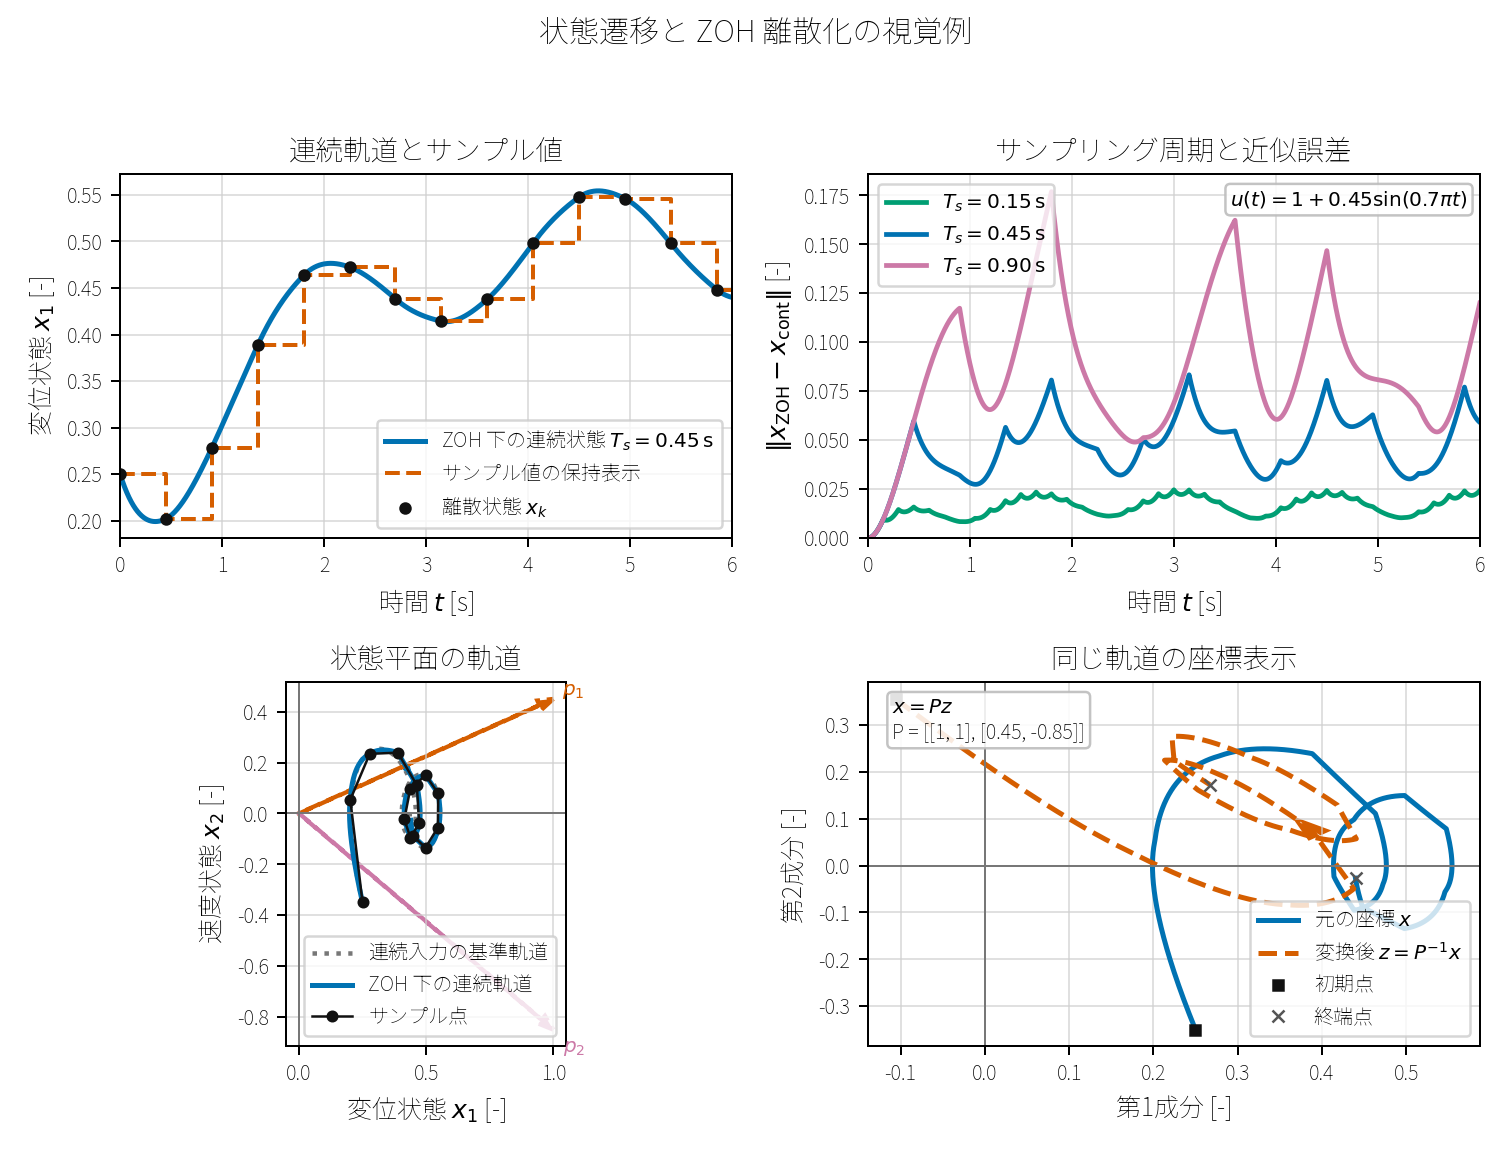
\includegraphics[width=0.96\linewidth,bb=0 0 1512 1152]{figures/state_transition_discretization_examples.png}
\caption{二状態モデルにおける状態遷移、ZOH 離散化、サンプリング周期、座標変換の関係。左上は ZOH 入力のもとで連続状態が曲線として動き、離散モデルはサンプル時刻の点列を与えることを示す。右上は滑らかな入力を ZOH 入力で近似したときの状態誤差であり、$T_s$ が大きいほど保持入力の粗さが状態へ残る。左下は同じ現象を状態平面上の軌道として表し、右下は $P=\left[\begin{smallmatrix}1&1\\0.45&-0.85\end{smallmatrix}\right]$ とした $x=Pz$ による別の基底で同じ軌道を表示している。}
\label{fig:state-transition-discretization-examples}
\end{figure}

図\ref{fig:state-transition-discretization-examples} の左上で曲線と黒点が一致するのは、\weq{zoh-exact-discretization} が ZOH 入力のもとでサンプル時刻の状態を厳密に写しているためである。階段状の線は、状態そのものが階段状に動くという意味ではなく、サンプル値だけを次のサンプルまで保持して表示したものである。実際の連続時間対象は、保持された入力を受けながら区間内でも $e^{A(t-t_k)}x_k+\int_0^{t-t_k}e^{A\sigma}B\,\dd\sigma\,u_k$ に従って動き続ける。

右上の誤差は、連続入力 $u(t)$ をそのまま加えた基準軌道と、$u_k=u(t_k)$ を区間内で保持した ZOH 軌道との差である。$T_s$ を小さくすると入力の保持区間が短くなり、連続入力に近い軌道になる。$T_s$ を大きくすると計算回数は減るが、入力更新の遅れと保持誤差が大きくなり、サンプル点では妥当に見える離散モデルでもサンプル間の連続状態が設計意図から離れることがある。したがって離散化では $A_d,B_d$ の計算だけでなく、入力がどの周期で更新され、サンプル間の状態をどの程度まで無視できるかを確認する。

右下は、同じ連続軌道を別の基底で表示した例である。ここで用いる座標変換行列を
\begin{equation}
  P=\begin{bmatrix}
    1&1\\
    0.45&-0.85
  \end{bmatrix}
  =\begin{bmatrix}p_1&p_2\end{bmatrix},\qquad
  p_1=\begin{bmatrix}1\\0.45\end{bmatrix},\quad
  p_2=\begin{bmatrix}1\\-0.85\end{bmatrix}
  \label{eq:state-transition-coordinate-p}
\end{equation}
と定義する。$x=Pz$ とおけば、連続時間モデルは
\begin{equation}
  \dot{z}=P^{-1}APz+P^{-1}Bu
\end{equation}
となり、ZOH 離散モデルは
\begin{equation}
  z_{k+1}=P^{-1}A_dPz_k+P^{-1}B_d u_k
  \label{eq:coordinate-transformed-discrete-model}
\end{equation}
となる。軌道の図形は座標成分の取り方で変わって見えるが、同じ物理状態を表している。可制御性、可観測性、安定性のような性質を座標変換で失ってはならないので、後で正準形や極配置を扱うときは、どの座標で設計し、元の座標へどう戻すかを明示する。

\begin{practice}[状態遷移、ZOH、座標変換の確認]
図\ref{fig:state-transition-discretization-examples} と同じ
$A=\left[\begin{smallmatrix}0&1\\-2&-3\end{smallmatrix}\right]$、
$B=\left[\begin{smallmatrix}0\\1\end{smallmatrix}\right]$ について、$T_s=0.45$ として $A_d=e^{AT_s}$ と $B_d=\int_0^{T_s}e^{A\sigma}B\,\dd\sigma$ を数値で求めよ。初期値 $x_0=\left[\begin{smallmatrix}0.25&-0.35\end{smallmatrix}\right]^\T$、入力 $u_0=1$ を用いて、$k=0$ から一歩後のサンプル状態 $x_{k+1}=A_dx_k+B_du_k$ を計算し、図の最初のサンプル点が連続軌道上にある理由を説明せよ。さらに \weq{state-transition-coordinate-p} の $P$ で $x=Pz$ とおいたとき、\weq{coordinate-transformed-discrete-model} の $P^{-1}A_dP$ と $P^{-1}B_d$ を計算し、同じ物理状態が異なる座標成分で表されることを確認せよ。
\end{practice}
